% ---------------------------------------------------------------------------- 
% 
% $Description: Slides presentation using Beamer $
% 
% $Author: dloubach $
% $Release Date: September 28, 2015 $
% 
% This was first used in the Technical Discussions Seminar of our lab:
% Advanced Computing, Control & Embedded Systems Laboratory
% http://www.fem.unicamp.br/~acceslab
% 
% ------------------------------------------------------------------------- 

\documentclass{beamer}
\mode<presentation>
{
  \usetheme{PaloAlto} %other templates i like: Hannover, Berkeley, PaloAlto
  \setbeamercovered{transparent}
  \usecolortheme{seahorse}
}

\synctex=1

% kind of 'minimum' packages to use
\usepackage{times}
\usepackage[english]{babel} % or portuguese
\usepackage[utf8]{inputenc} % or latin1
\usepackage[T1]{fontenc}
\usepackage{graphicx}
\graphicspath{{./figs/}}

\usepackage{array}
\usepackage{tabularx}
\usepackage{booktabs}
\usepackage{colortbl}

\usepackage{multicol}
\usepackage{setspace}
\usepackage{pifont}
\usepackage{overpic}
\usepackage{listings}

% for math 
\usefonttheme[onlymath]{serif}

% listing for C language
\lstset{language=C,
  basicstyle=\ttfamily,
  keywordstyle=\color{blue}\ttfamily,
  stringstyle=\color{red}\ttfamily,
  commentstyle=\color{cyan}\ttfamily\textbf,
  % morecomment=[l][\color{gray}]{\#},
  showstringspaces=false
}

% navigation symbols
\setbeamertemplate{navigation symbols}
{
  \insertslidenavigationsymbol 
  \insertframenavigationsymbol   
  \insertsubsectionnavigationsymbol  
  \insertsectionnavigationsymbol
  \insertdocnavigationsymbol  
  \insertbackfindforwardnavigationsymbol 
  \hspace{1em}
  \usebeamerfont{footline}
  \insertframenumber/\inserttotalframenumber
}



% presentation title
\title[SDT ACCES-Lab]{Research Presentation}
\subtitle[*]{\LaTeX-based Example}

% author info
\author[Surname, Name]{
  \textbf{Author Name}\\
  \tiny{[[Master|PhD] student | Professor]] \\
    email@provider.br} \\
}

% institute
\institute[ACCES-Lab]{
  \textit{Advanced Computing, Control \& Embedded Systems Laboratory}\\
  Universidade Estadual de Campinas - UNICAMP
  
  \begin{figure}[h!]
    \centering
    
\includegraphics[scale=.40]{acces_logo_peq}
    
\includegraphics[scale=.20]{logo_unicamp}
  \end{figure}
}

\date{\tiny September, 28 2015}

\pgfdeclareimage[width=0.110\textwidth]{university-logo}{figs/acces_logo_peq}
\logo{\pgfuseimage{university-logo}}

\makeatletter
\makeatother



\begin{document}

\frame{\titlepage}

\section[]{}
\frame{\frametitle{Agenda} \small \tableofcontents}

\section{Motivation}
\frame{
  \frametitle{Motivation}
  \small
  \begin{figure}[h!]
    \centering
    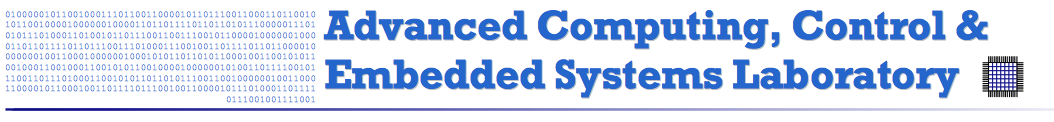
\includegraphics[scale=.45]{acces_logo}
  \end{figure} 
  
  \begin{quotation}
    Give your research context here
  \end{quotation}
  
  \begin{itemize}
  \item \vfill Why this subject is relevant?
  \item \vfill What are the main drawbacks of it?
  \end{itemize}
}

\section{Research Goal}
\frame{
  \frametitle{Research Goal}
  \small

  \begin{enumerate}
  \item \vfill Clearly state your research goal
  \item \vfill \pause You may also give a research question in here
  \item \vfill \pause And, your expected contributions to your research area
  \end{enumerate}

}

\section{Development \& Methods}
\frame{
  \frametitle{Development \& Methods}
  \small

  Present you development here

  \vfill
  Which methods have you used to go through your research?

}

\section{Results and Discussions}
\frame{
  \frametitle{Results}
  \small
  \begin{itemize}
  \item Which results did you achieved?
  \item \pause Are they preliminary, final? Explain them all
  \end{itemize}		

}

\section{Conclusion}
\frame{
  \frametitle{Conclusion}
  \small
  Respond to your research question here, \emph{i.e.}, which was your
  contribution and work limitations
}


\section{References}
\frame{
  \frametitle{References}
  
  \scriptsize
  Never forget to cite your sources...
  
  \nocite{Ganssle:2000aa, Liu:1973aa, Douglass:2003aa}

  \vfill
  \begingroup
  \renewcommand{\section}[2]{} %remove o nome da seção (References ou Referências) 
  \bibliography{refs/my-refs}
  \bibliographystyle{ieeetr}
  \endgroup
}

\section{Questions \& Answers}
\frame{
  \frametitle{Questions \& Answers}
  \small
  \begin{quotation}
  Prepare for the worst, hope for the best!\\    
  \end{quotation}
  \flushright
  Benjamin Disraeli
}

\frame{
  \frametitle{Enjoy your research}
  \small
  
  \begin{figure}[h]
    \centering
    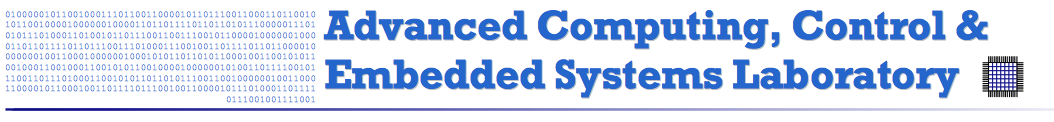
\includegraphics[scale=0.50]{acces_logo}\\%
    \tiny
    \url{http://www.fem.unicamp.br/~acceslab}    		
  \end{figure}
}

\end{document}

%%% Local Variables:
%%% mode: latex
%%% TeX-master: t
%%% End:
